\chapter{Mengenal Kecerdasan Buatan dan Scikit-Learn}

\section{Teori}
\begin{enumerate}
\item Definisi, Sejarah dan perkembangan Kecerdasan Buatan.\\
Kecerdasan merupakan kemampuan untuk memahami dan melakukan sesuatu secara cepat dan tepat.\\
Kecerdasan Buatan merupakan sebuah sistem yang dibuat untuk dapat memahami dan melakukan sesuatu seperti memberikan keputusan, melakukan pencarian, dan mengelompokkan sesuatu dengan cepat dan tepat. Sistem ini diharapkan memiliki kecerdasan layaknya manusia.\\
Pada tahun 1943 – 1956 McCulloch dan Walter Pitts memahami pengathuan fisiologi dasar dan fungsi sel saraf dalam otak dan adanya penelitian yang dilakukan oleh seorang pionir AI dan ahli matematika inggris, Alan Turing melakukan sebuah percobaan yang dikenal dengan turing test, dalam percobaannya ia membuat sebuah software yang memungkinkan seseorang dapat berkomunikasi, seorang operator dalam percobaan itu mengira bahwa dirinya sedang berkomunikasi dengan seorang manusia (operator lainnya) padahal dalam kenyataannya seorang operator tersebut berkomunikasi dengan komputer.Intinya pada masa ini mereka berhasil membuat sistem saraf tiruan.\\
Setelah itu McCarthy berhasil menemukan program numerik dan menyelesaikan masalah yang dinamai principia mathematica, oleh karena itu McCarthy dikenal sebagai the father of AI. Kemudian AI memasuki masa perkembangan, saat itu Newell dan Simon membuat sebuah program bernama General Problem Solver yang mampu menyelesaikan permasalahan seperti manusia. Setelah itu McCarthy menemukan sebuah bahasa pemrograman LISP untuk pembuatan program AI dan ia membuat sebuah program pencarian solusi dari permasalahan menggunakan pengetahuan yang disebut Program with Common Sense. \\ 
Pada tahun 1969-1979, adalah masa perkembangan sistem berbasis pengetahuan, pada masa ini Ed Feigenbaum, Bruce Buchanan, dan Joshua Lederberg menemukan sebuah program bernama Dendral Programs, program ini mampu memecahkan masalah molekuler, kemudian ditemukan juga Computer Biomedicine, yaitu sistem diagnosa penyakit menggunakan AI.\\
Pada tahun 1980-1988, AI menjadi sebuah industri. pada masa ini terdapat penemuan expert system yang dinamakan R1.\\
Pada tahun 1986 – sekarang ini, merupakan era jaringan syaraf tiruan, terdapat penemuan algoritma Back Propagation Learning yang telah diimplementasikan ke dalam bidang ilmu komputer dan psikologi.

\item Definisi supervised learning, klasifikasi, regresi dan unsupervised learning. Data set, training set dan testing set.\\

Supervised Learning merupakan algoritma yang digunakan untuk menentukan prediksi dan klasifikasi yang mana variabel x dan variabel y telah diketahui sebelumnya. algoritma ini seolah-olah dilatih untuk menentukan prediksi dan klasifikasi tersebut.\\

klasifikasi adalah pengelompokkan sesuatu berdasarkan kelas-keasnya, persamaan ciri dan perbedaannya.\\

regresi merupakan suatu metode analisis yang digunakan dalam statistika, metode ini berguna untuk melihat pengaruh antara dua variabel atau lebih.\\

unsupervised learning merupakan algoritma yang mana dalam menentukan suatu prediski atau klasifikasi tidak memerlukan target variabel, variabel hanya berupa x dan y saja.\\

Data set merupakan sekumpulan data yang akan diinputkan dan diproses, dapat berupa record, point, vector, pattern, observation, case, dll.\\

Training set merupakan bagian dari data set yang dilatih untuk membuat sebuah prediksi dan klasifikasi.\\

testing set adalah bagian dari data set yang akan di testing, testing dilakukan untuk melihat seberapa akurat hasil prediski dari data tersebut.\\

\end{enumerate}

\section{Instalasi}
\begin{enumerate}
\item
Instalasi library scikit dari anaconda, mencoba kompilasi dan uji coba ambil contoh kode dan lihat variabel explorer.\\

\begin{figure}
    \centering
    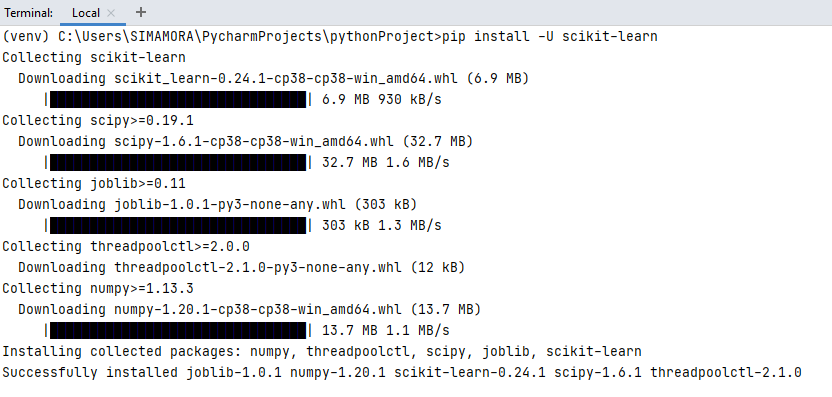
\includegraphics[width=12cm,height=6cm]{figures/1.PNG}
    \caption{Instalasi Library Scikit-Learn}
    \label{fig:my_label}
\end{figure}

\begin{figure}
    \centering
    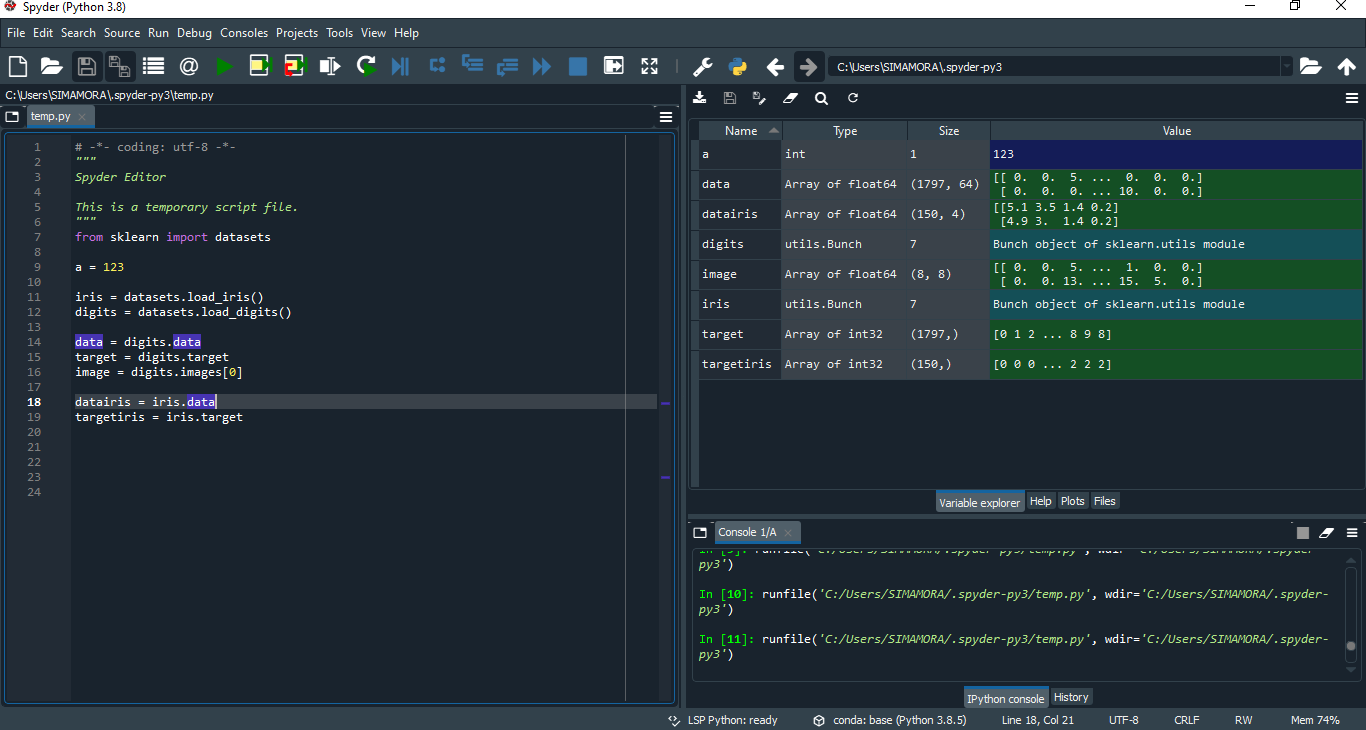
\includegraphics[width=12cm,height=6cm]{figures/ve.PNG}
    \caption{Variable Explorer}
    \label{fig:my_label}
\end{figure}

\item
Mencoba Loading an example dataset, menjelaskan maksud dari tulisan tersebut dan mengartikan per baris.\\

Loading an example dataset (memuat contoh kumpulan data) maksudnya yaitu scikit-learn memugkinkan kita untuk mengambil atau memuat data standar, misalnya kita mengambil atau memuat data set iris dan digits untuk membuat sebuah klasifikasi dan data set diabetes untuk regresi.\\

\begin{lstlisting}[language=Python]
def loadingAnExample():
    iris = datasets.load_iris()
    digits = datasets.load_digits()
    print(digits.images[0])
\end{lstlisting}

\item
Mencoba Learning and predicting, menjelaskan maksud dari tulisan tersebut dan mengartikan per baris.\\

Learning and Predicting (Belajar dan Memprediksi) maksudnya yaitu belajar dari sebuah model dan membuatkan prediksi dalam sebuah gambar. Menggunakan data set digits karena data digits dapat memprediksi, mengingat gambar digit mana yang diwakilinya. \\

\begin{lstlisting}[language=Python]
def learningAndPredicting():
    digits = datasets.load_digits()
    clf = svm.SVC(gamma=0.001, C=100.) #parameter model

    data = clf.fit(digits.data[:-1], digits.target[:-1]) #fit x, y
    print(data)

    prediksi = clf.predict(digits.data[-1:]) #predict T (hasil prediksi data baru)
    print(prediksi)
\end{lstlisting}

\item
mencoba Model persistence, menjelaskan maksud dari tulisan tersebut dan mengartikan per baris.\\
Model Presistence maksudnya mempertahankan sebuah model agar bisa digunakan di masa depan tanpa perlu melatih kembali atau membuat model itu kembali. Menyimpan model dengan menggunakan pickle atau joblib

\begin{lstlisting}[language=Python]
def modelPresistence():
    clf = svm.SVC()
    X, y = datasets.load_iris(return_X_y=True)
    print(clf.fit(X, y))

    #contoh menggunakan pickle
    s = pickle.dumps(clf)
    clf2 = pickle.loads(s)
    print(clf2.predict(X[0:1]))

    print(y[0])

    #contoh menggunakan joblib
    to_persist = [('a', [1, 2, 3]), ('b', np.arange(10))]
    dump(to_persist, 'filename.joblib')

    # dump(clf, 'filename.joblib')
    # clf = load('filename.joblib')

    print(load('filename.joblib'))
\end{lstlisting}

\item 
Mencoba Conventions, menjelaskan maksud dari tulisan tersebut dan mengartikan per baris.\\

Conventions (konvensi) maksudnya dapat memprediksi dengan lebih prediktif.\\

\begin{lstlisting}[language=Python]
def conventions():
    #type casting
    rng = np.random.RandomState(0)
    X = rng.rand(10, 2000)
    X = np.array(X, dtype='float32')
    print(X.dtype) #type float 32

    transformer = random_projection.GaussianRandomProjection()
    X_new = transformer.fit_transform(X)
    print(X_new.dtype) #type float 64

    # jika type tidak ditentukan, maka akan diformat langsung ke type float 64
    iris = datasets.load_iris()
    clf = SVC()
    print(clf.fit(iris.data, iris.target))

    print(list(clf.predict(iris.data[:3])))

    print(clf.fit(iris.data, iris.target_names[iris.target]))

    print(list(clf.predict(iris.data[:3])))

    #Refitting and updating parameters
    #memperbaiki dan memperbarui parameter
    X, y = load_iris(return_X_y=True)

    print(clf.set_params(kernel='linear').fit(X, y))
    print(clf.predict(X[:5]))

    print(clf.set_params(kernel='rbf').fit(X, y))
    print(clf.predict(X[:5]))

    #Multiclass vs. multilabel fitting
    X = [[1, 2], [2, 4], [4, 5], [3, 2], [3, 1]]
    y = [0, 0, 1, 1, 2]

    classif = OneVsRestClassifier(estimator=SVC(random_state=0))
    print(classif.fit(X, y).predict(X)) #klasifikasi array 1 dimensi

    # klasifikasi array 2 dimensi yang mewakili prediksi multilabel
    y = LabelBinarizer().fit_transform(y)
    print(classif.fit(X, y).predict(X))

    # klasifikasi array 2 dimensi dengan beberapa label yang diprediksi untuk setiap instans.
    y = [[0, 1], [0, 2], [1, 3], [0, 2, 3], [2, 4]]
    y = MultiLabelBinarizer().fit_transform(y)
    print(classif.fit(X, y).predict(X))
\end{lstlisting}

\end{enumerate}


\section{Penanganan Error}
Dari percobaan yang dilakukan di atas, apabila mendapatkan error maka:

\begin{enumerate}
	\item
	skrinsut error[hari ke 2](10)
	\item
Tuliskan kode eror dan jenis errornya [hari ke 2](10)
	\item
Solusi pemecahan masalah error tersebut[hari ke 2](10)

\end{enumerate}

